\chapter{FSServer}
\label{chap:fsserver}
This chapter deals with the requirements specification, analysis, design and non-trivial implementation details of FSServer.

\section{Requirements Specification}

The requirements for FSServer are:

\begin{itemize}
	\item must be installed on GS
	\item must accept TCP connection
	\item must send failsafe commands via the datalink
	\item must send failsafe responses back to TCP clients
	\item must ensure atomicity of failsafe commands
\end{itemize}

In addition to these requirements, the following requirements was identified when the overall design was agreed upon:

\begin{itemize}
	\item must run as a daemon and log all activity to a file
	\item must execute scripts on GS and from a TCP client and immediately send any response back to the TCP client
	\item must validate failsafe commands
\end{itemize}









\section{Analysis and design}
Lets go through the requirements one by one. For each requirement we will enhance the design to incorporate the requirement.

\textbf{Must be installed on GS} \\
Trivial constraint.

\textbf{Must accept TCP connections} \\
Clients can connect to the server with the TCP protocol over an internet socket.
The server could accept one or multiple connections at a time. We want to ensure that only one command is send to the satellite at a time, so lets accept only one connection for now.

\textbf{Must send failsafe commands via the datalink and send response back to clients} \\
We could implement pull-behaviour where each request is answered with exactly one response or we could implement push-behaviour where data can be pushed to the client without being requested. It is not obvious which of these behaviours we should implement so lets choose the pull-behaviour for now.

\textbf{Must ensure atomicity of failsafe commands} \\
Only one satellite command can be executed at a time. If we use a request queue with atomic enqueue and dequeue operations we can implement this behaviour without race conditions.

\textbf{Must run as a daemon and log all activity to a file} \\
A unix daemon is a process with a parent process id of 1. When starting the server, the staff must be able to decide whether to run it as a daemon or to run it as a normal process.
The logfile could be a predefined file, but we should let the staff decide by providing an option when starting the server.

\textbf{Must execute scripts on GS and from a TCP client and send any response back to the TCP client} \\
Some tasks, such as uploading a binary file to the satellite, are so common that they should be available for every client. Instead of implementing these tasks in every client, the server should implement them and execute them when requested by the client.
The scripts can be written in any language that is supported by the server environment. To capture the output of a script, the server will open a pseudo terminal that has control of standard output and input. The script is executed in the pseudo terminal and any output can be send to the client.

\textbf{One or multiple TCP connection} \\
Now consider the following scenario. A client connects to the server and requests to execute script X. Because of the pull behaviour we decided upon earlier the client will now wait for the script to finish with the response. If script X needs to interact with the satellite, it must connect to the server and do some requests but the server only accepts one TCP connection at a time, and we have a deadlock situation.

\begin{figure}[h!] \centering
	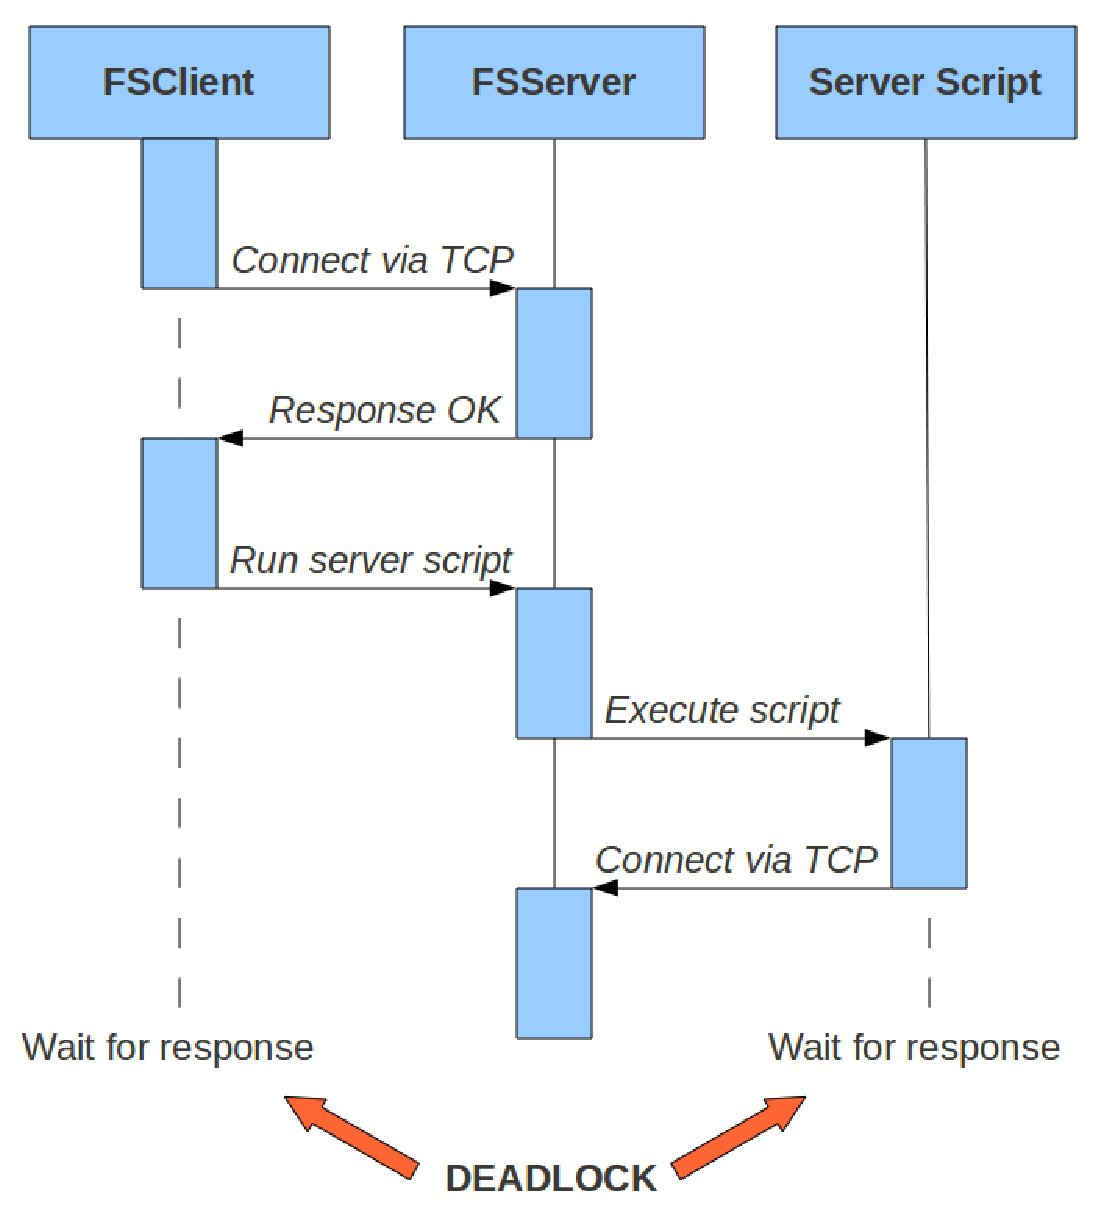
\includegraphics[scale=0.5]{img/one_connection_deadlock}
  \caption{Deadlock when executing script}
\end{figure}

So there is a need for handling multiple TCP clients and their requests simultaneously. Satellite commands over the serial connection must not be simultaneous however!

\textbf{Blocking vs. non-blocking execution} \\
In a program a non-blocking execution of a statement will not wait for the result of that statement before proceeding with the execution of the next statement. A blocking execution of a statement will wait for the result before proceeding.
In order to handle multiple TCP clients concurrently the server must execute the requests in a non-blocking fashion.

\textbf{Lock mechanism} \\
With multiple clients new concerns must be dealt with. Consider the scenario where two clients execute a server script each. The script consists of 2 satellite commands and although we can ensure that only one satellite command are being executed at a time, we can not ensure that the 2 commands are executed sequentially.

\begin{figure}[h!] \centering
	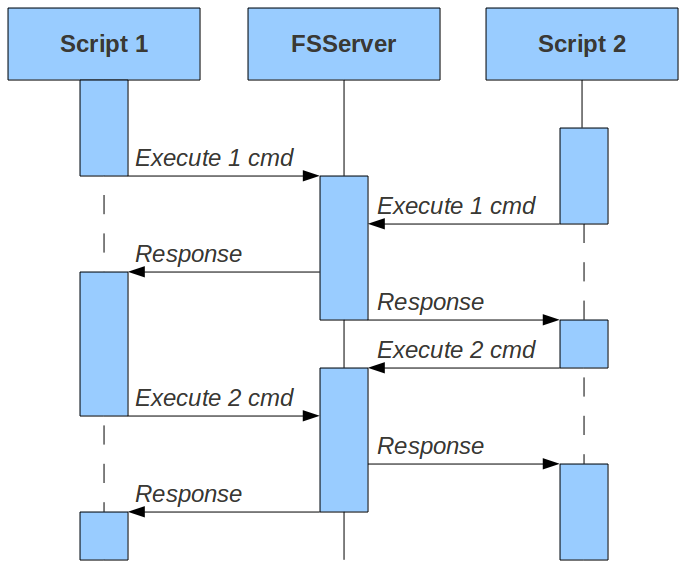
\includegraphics[scale=0.5]{img/multiple_scripts_no_lock}
  \caption{Two scripts executing without locking}
\end{figure}

We need a way to lock the server to prevent multiple executing scripts from stepping on each others toes. So after connecting to the server a client must first issue a lock request and will receive a session token if the lock succeeded or a message indicating that the server is already locked.

When finished an unlock request can be sent to unlock the server. Things can go wrong however and leave the server in a locked state, so there will be implemented a timeout on the token. After each request this timeout will be reset. If the token gets timed out, a broadcast message will be sent to all connected clients.
It is important to note that two scripts requested by clients using the same token will be executed simultaneously!

\begin{figure}[h!] \centering
	
\includegraphics[scale=0.5]{img/lock}
  \caption{Two scripts executing with locking}
\end{figure}

\textbf{Partial responses} \\
Another thing to consider is the output of the server scripts. Imagine for instance an upload script that prints to standard out each time 10\% of the upload is done. The client would like to follow this progress in real time as opposed to seeing the total output of a script when execution has finished. So in the case of the upload script we would at least be sending 10 partial messages in response to one request.
This along with the timeout broadcast leads to the need for pushing data to clients and we must therefore implement the push-behaviour in favor of the pull-behaviour.

\begin{figure}[h!] \centering
	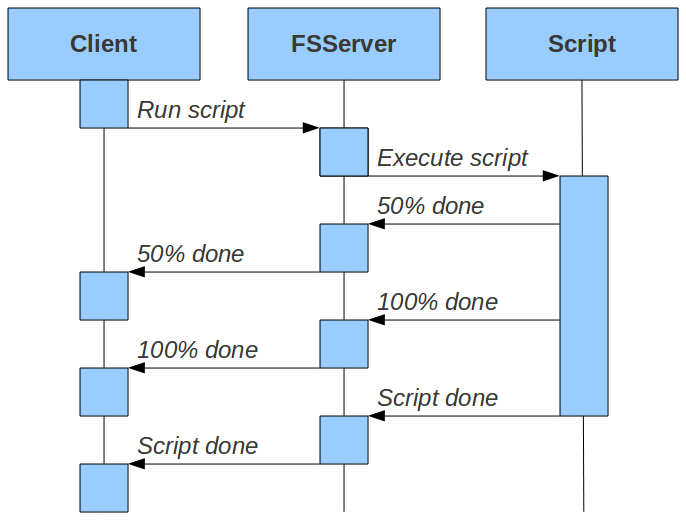
\includegraphics[scale=0.5]{img/partial_responses}
  \caption{Partial response}
\end{figure}

\textbf{Must validate failsafe commands} \\
Failsafe commands can have arguments such as "address", "length" etc. These arguments must be validated before being send to the satellite. Arguments are typically memory addresses and other hexadecimal values. It would be convenient to use both hexadecimal ("0xff") and decimal ("255") values as arguments. If an argument is invalid or missing the client must be informed and the request must not be executed.

\subsection{Data format}
Now that we have a design that covers all features, lets look at the data format. We have several choices here. We could go with a simple text format, XML or JSON.

The client must be able to send a message to the server and react to the received response. There must be a way of determining whether incoming data is a response to some outgoing data. As there are no such information in the order of the outgoing and the incoming data, a request must be stamped with a unique identification key that can be used by the server to stamp the response. The data format must at least have two parameters then, a stamp and the data.

If we use a simple text format we would need a separator to distinguish the parameters. Then we would have to care about escaping certain characters etc. Instead we should consider using the semantically equal XML or JSON formats. We will be using JSON.

\begin{itemize}
	\item Request: \texttt{\{"id":KEY, "data":REQUEST\}}
	\item Response: \texttt{\{"id":KEY, "data":RESPONSE\}}
\end{itemize}
Example of a "lock" request:
\begin{itemize}
	\item Request: \texttt{\{"id":"1","data":"lock"\}}
	\item Response: \texttt{\{"id":"1","data":"7KFdnNXBYi8nmuWV"\}}
\end{itemize}

If the client has locked the server, the token is sent along the request like this:

\begin{itemize}
	\item Request: \texttt{\{"id":"1","data":"reset","token":"7KFd"\}}
\end{itemize}

Besides from being able to respond to incoming requests, the server also needs to push data to the client independently of any requests. The client must be able to determine the data type to handle it correctly. The format must at least look like:

\begin{itemize}
	\item Message: \texttt{\{"type":TYPE\}}
\end{itemize}

Example of an "token timout" message:

\begin{itemize}
	\item Message: \texttt{\{"type":"server\_unlocked"\}}
\end{itemize}

For format consistency and faster processing on the client side, the response format will also have the type parameter:

\begin{itemize}
	\item Response: \texttt{\{"type":"response", "id":KEY,"data":RESPONSE\}}
\end{itemize}

The server must also be able to send more than one response to a given request. This can be solved with the following format:

\begin{enumerate}
	\item Req: \texttt{\{"id":"2", "data":"run\_script upload filepath", "token":"7KFd"\}}
	\item Res: \texttt{\{"type":"response", "id":"2", "data":"50\% done", "partial":"true"\}}
	\item Res: \texttt{\{"type":"response", "id":"2", "data":"100\% done", "partial":"true"\}}
	\item Res: \texttt{\{"type":"response", "id":"2", "data":""\}}
\end{enumerate}

























\section{Implementation}
This section deals with the non-trivial implementation details.

\textbf{Language and libraries} \\
There are no contraints to the programming language and as the server will neither be cpu- or io intensive the server has been implemented in Ruby. It could have been implemented in C or Java, and probably should have if there where any requirements to speed.

Ruby has a standard library with support for basic things like sockets, threads, system etc. There is a packaging tool called rubygems with which one can install third party libraries called gems.

Instead of reinventing a TCP server, a serialport wrapper and a JSON parser we will be using production ready ruby gems that has been tested over long periods of time by many people and have been accepted within the ruby community.

Third-party gems used in the implementation:
\begin{itemize}
	\item \textbf{Eventmachine} - Instead of the relatively slow socket support in the standard library we will be using the evetnmachine gem. Eventmachine is a library for implementing non-blocking TCP servers and clients.
	\item \textbf{JSON} - provides a JSON parser class.
	\item \textbf{Serialport} - provides a class for using RS-232 serial ports.
	\item \textbf{Daemons} - provides an easy way to wrap existing ruby scripts to be run as a daemon and to be controlled by simple start/stop/restart commands.
\end{itemize}



\textbf{Safe script execution} \\
When executing server scripts from a client we must be very careful about the parameters. Consider the scenario were a client sends this request:
\begin{verbatim}
	run_script scriptname param1;rm -rf}
\end{verbatim}
If we are not careful and just pass along the parameters without escaping the semicolon, the result of this command will delete all files on the server, that the currently running user has permissions for.

Ruby has a wrapper for the UNIX command execve. Execve can create new UNIX processes and will safely pass arguments along.
Ruby's pseudo tty library uses the execve wrapper to execute console commands.

\textbf{Failsafe Commands} \\
A failsafe command is a Ruby class that can have an initialize, a validate and an execute method. Initialize takes the arguments for the command, validate will validate the arguments and execute will execute the command.

All commands inherits common code from the AbstractCommand class. This class implements some common validations, a default initialize method, a default validate method and a default execute method.

\textbf{Parsing} \\
When the server gets a new request, it is parsed with the JSON gem. The id and token are easily looked up in the resulting Ruby hash. The data field is first split on spaces to separate the command from its arguments. The command is then camelized which means that the first character and any characters immediately after an underscore is capitalized. The underscores are then removed. Each command has a corresponding camelized Ruby class.

For example: \\
The server receives this request:
\begin{verbatim}
	{"id":"1","token":"abcdefg", "data":"run_script filepath arg1 arg2"}
\end{verbatim}

First it is parsed as JSON. This results in a Ruby hash where we immediately lookup the id and the token. The data is then split on spaces:

\begin{verbatim}
	cmd, *arguments = parsed_request["data"].split
\end{verbatim}

Ruby has a function called eval that takes a string as a parameter and executes that string as Ruby code. To get an instance of the camelized class to a run\_script command we can execute the following:

\begin{verbatim}
	eval(cmd.camelize+".new(*arguments)")
\end{verbatim}

which is equivalent to:

\begin{verbatim}
	eval("RunScript.new(*arguments)")
\end{verbatim}

When this string is executed by eval, the initialization code for RunScript will be called with all the arguments.

Options are also extracted. If an argument begins with a dash ("-") then it will be split on equal-signs and stored in an options hash.

Again we must be very careful when executing a string from an unknown place. In this way a user could create an instance of any Ruby class and pass any arguments to it. To deal with this, we encapsulate all valid commands in a module called Commands. So now the eval looks like:

\begin{verbatim}
	eval("Commands::#{cmd.camelize}.new(*arguments)")
\end{verbatim}

\textbf{Validation} \\
When the command has been parsed the server will call the validate method before calling the execute method. If the validate method fails the execute method will never be called, instead a failed validation message is sent to the client.

Common validations are implemented in the AbstractCommand class and uses some extensions to the String class. The most common validation is to ensure that the argument is addressable. To be addressable the value must be given as a hex or a decimal value. The validation ensures that the value is not greater than 0xffffffff.

\textbf{Satellite IO} \\
The server will have to communicate with the radio link on GS when communicating with the satellite. During development however a development board has been used. This board has a RS-232 interface, so the serialport gem has been used to write an serialport implementation that adheres to the protocol layer interface.

\textbf{Request queue with atomic enqueue and dequeue operations} \\
It is important that only one command is being sent at any given time to the satellite. Therefore, a ProcessingQueue module has been implemented. A processing queue has an array of requests, a mutex and a boolean value to indicate that the processing has already started. When enqueueing, the request is put into the queue when the mutex becomes available. Then the processesing loop is started unless it has already been started.

The queue is when the mutex becomes available and the request is processed. As soon as the processing is done the mutex is released and the processing is started again until there is no more requests left in the queue.

Option for satellite commands:
\begin{itemize}
	\item \textbf{--timeout=SEC} - There is a timeout for each executing satellite command. It is set to 5 seconds by default but can be changed per request with the timeout options e.g. "reset" and "reset --timeout=20" are both valid commands. The former will timeout after 5 seconds and the latter will timout after 20 seconds.
	\item \textbf{--no-response} - Sometimes we do not care about the response for a command and would like to skip it in order to save execution time and batterylife. The option looks like this: "reset -no-response".
\end{itemize}

\textbf{Broadcasting} \\
Broadcasting can be done by maintaining a global array of connected clients. A message can then be sent to each client.

\textbf{Token handling and timeout} \\
The TokenHandler class is responsible for timing out the token. It has a token variable, which is just a string. The server is unlocked if this value is nil. When setting the token variable a timer will be started. If the timer runs out the token variable will be set to nil and a broadcast message is sent to all connected clients.

\textbf{Logging} \\
When starting the server one can indicate to use a logfile for the server output. If none is indicated the server will print its output to standard out.
